\section{Component-Wise Performance Evaluation of OLTP Systems}

\frame{\sectionpage}

\subsection[OLTP through the Looking Glass, and What We Found There]{OLTP through the Looking Glass, and What We Found There \cite{Harizopoulos:2008}}

\frame{\subsectionpage}

\begin{frame}
    \centering
    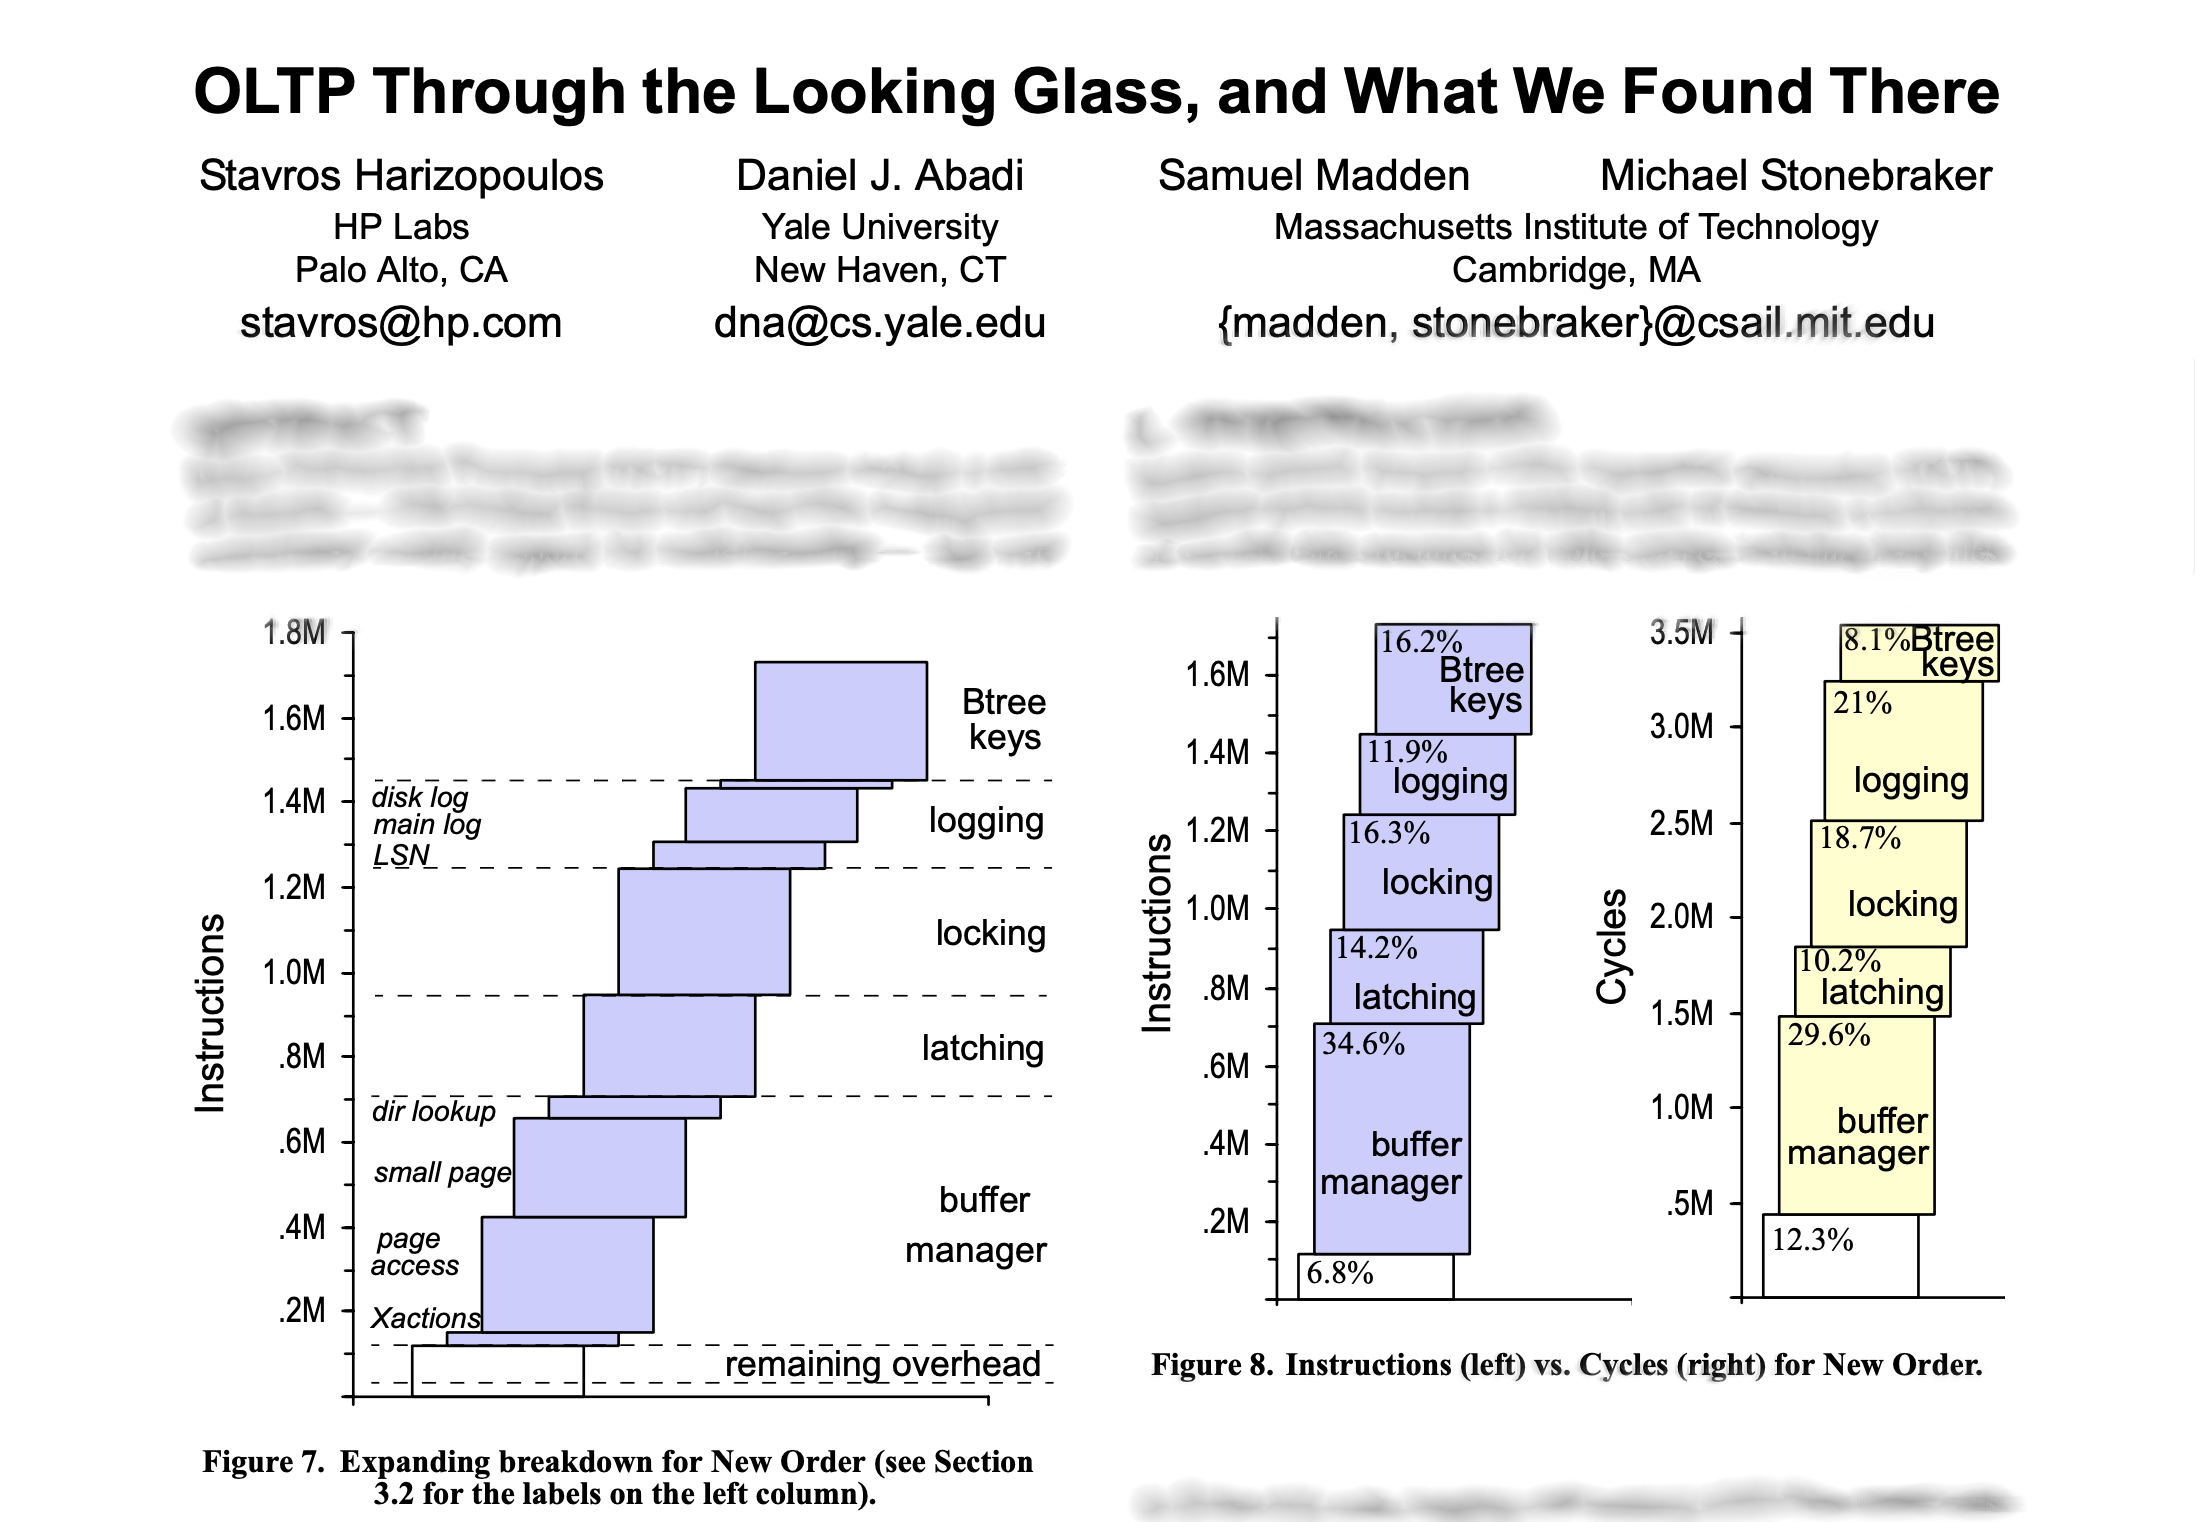
\includegraphics[width = \linewidth]{data/oltp_through_the_looking_glass.png}
\end{frame}

\begin{frame}
    \frametitle{The Author's Assumptions}

    \begin{itemize}
        \item<2->   No more larger-than-memory DBs
        \item<3->   Thus, multithreaded and interleaved transaction execution no more needed
        \item<4->   Many applications do not need ACID transactions
        \item<5->   Replication instead of logging for recovery
    \end{itemize}
\end{frame}

\begin{frame}
    \frametitle{The Author's Methodology}
    
    \uncover<2->{Gradually ...}
    \begin{itemize}
        \item<3->   ... make the DBS in-memory---removing buffer pool---, ...
        \item<4->   ... remove latching \uncover<5->{and locking, ...}
        \item<6->   ... remove transaction logging and LSN maintenance, ...
        \item<7->   ... and hand-optimize B-tree code for in-memory DBS.
    \end{itemize}
\end{frame}

\subsection{Results}

\frame{\subsectionpage}

\begin{frame}
    \frametitle{Read-Only YCSB}

    \pgfplotsset{%
        every axis/.append style = {
            ybar stacked,
            ylabel near ticks,
            y label style = {font = \small},
            ylabel shift = -.5em,
            ymode = normal,
            ymin = 0,
            ymax = 100,
            yticklabel style = {font = \scriptsize},
            ymode = normal,
            scaled y ticks = false,
            xmin = -0.25,
            xmax = 0.25,
            xtick = \empty,
            bar width = 0.5,
            ymajorgrids = false,
            width = .2875\textwidth,
            height = .85\paperheight
        }
    }

    \tikzset{%
        a0/.style = {black, fill = Cerulean},
        a1/.style = {black, fill = Cerulean!80},
        a2/.style = {black, fill = Cerulean!60},
        a3/.style = {black, fill = Cerulean!40},
        a4/.style = {black, fill = Cerulean!20},
        b0/.style = {black, fill = magenta},
        b1/.style = {black, fill = magenta!50},
        d/.style = {black, fill = white}
    }

    \Wider[6em]{%
        \centering
        \begin{tikzpicture}[remember picture,
                            visible on = <2->]
            \begin{axis}[ymax = 100]
                \node at ($(0, 0)!.5!(0, 8.27+0.13+4.44+4.14+5.30)$) {\makecell[c]{\contour{white}{Buffer pool}\\\footnotesize \contour{white}{\SI{22.28}{\percent}}}};
                \node at ($(0, 8.27+0.13+4.44+4.14+5.30)!.5!(0, 8.27+0.13+4.44+4.14+5.30+32.09+2.38)$) {\makecell[c]{\contour{white}{Locking}\\\footnotesize \contour{white}{\SI{34.47}{\percent}}}};
                \node at ($(0, 8.27+0.13+4.44+4.14+5.30+32.09+2.38)!.5!(0, 8.27+0.13+4.44+4.14+5.30+32.09+2.38+1.01)$) {\scriptsize\makecell[c]{\contour{white}{Logging \SI{1.01}{\percent}}}};
                \node at ($(0, 8.27+0.13+4.44+4.14+5.30+32.09+2.38+1.01)!.5!(0, 8.27+0.13+4.44+4.14+5.30+32.09+2.38+1.01+42.24)$) {\makecell[c]{\contour{white}{B-tree}\\\footnotesize \contour{white}{\SI{42.24}{\percent}}}};

                \addplot[d]                        coordinates       {(0, 0)};
                \addplot[a4]    coordinates       {(0, 8.27)};
                \addplot[a3]    coordinates       {(0, 0.13)};
                \addplot[a2]    coordinates       {(0, 4.44)};
                \addplot[a1]    coordinates       {(0, 4.14)};
                \addplot[a0]    coordinates       {(0, 5.30)};
                \addplot[b1]    coordinates       {(0, 32.09)};
                \addplot[b0]    coordinates       {(0, 2.38)};
                \addplot[a0]    coordinates       {(0, 1.01)};
                \addplot[b0]    coordinates       {(0, 42.24)};

                \coordinate (single0rest)            at (0.25, 0);
                \coordinate (single0bufferRest)      at (0.25, 8.27);
                \coordinate (single0bufferFreeList)  at (0.25, 8.27+0.13);
                \coordinate (single0bufferHashTable) at (0.25, 8.27+0.13+4.44);
                \coordinate (single0bufferFetching)  at (0.25, 8.27+0.13+4.44+4.14);
                \coordinate (single0bufferLatching)  at (0.25, 8.27+0.13+4.44+4.14+5.30);
                \coordinate (single0lockingRest)     at (0.25, 8.27+0.13+4.44+4.14+5.30+32.09);
                \coordinate (single0lockingLatching) at (0.25, 8.27+0.13+4.44+4.14+5.30+32.09+2.38);
            \end{axis}
        \end{tikzpicture}
        \hspace{.125em}
        \begin{tikzpicture}[remember picture,
                            visible on = <2->]
            \begin{axis}[ymax = 8.27+0.13+4.44+4.14+5.30+32.09+2.38]
                \node at ($(0, 8.27)!.5!(0, 8.27+0.13)$)  {\scriptsize\makecell[c]{\contour{white}{Free list \SI{0.13}{\percent}}}};
                \node at ($(0, 8.27+0.13)!.5!(0, 8.27+0.13+4.44)$) {\scriptsize\makecell[c]{\contour{white}{Hash table \SI{4.44}{\percent}}}};
                \node at ($(0, 8.27+0.13+4.44)!.5!(0, 8.27+0.13+4.44+4.14)$){\scriptsize\makecell[c]{\contour{white}{Fetching \SI{4.14}{\percent}}}};
                \node at ($(0, 8.27+0.13+4.44+4.14)!.5!(0, 8.27+0.13+4.44+4.14+5.30)$){\scriptsize\makecell[c]{\contour{white}{Latching \SI{5.3}{\percent}}}};
                \node[anchor = north, inner ysep = .5pt] at (0, 8.27+0.13+4.44+4.14+5.30+32.09+2.38){\scriptsize\makecell[c]{\contour{white}{Latching \SI{2.38}{\percent}}}};

                \addplot[a4] coordinates       {(0, 8.27)};
                \addplot[a3] coordinates       {(0, 0.13)};
                \addplot[a2] coordinates       {(0, 4.44)};
                \addplot[a1] coordinates       {(0, 4.14)};
                \addplot[a0] coordinates       {(0, 5.30)};
                \addplot[b1] coordinates       {(0, 32.09)};
                \addplot[b0] coordinates       {(0, 2.38)};

                \coordinate (single1rest)            at (-0.25, 0);
                \coordinate (single1bufferRest)      at (-0.25, 8.27);
                \coordinate (single1bufferFreeList)  at (-0.25, 8.27+0.13);
                \coordinate (single1bufferHashTable) at (-0.25, 8.27+0.13+4.44);
                \coordinate (single1bufferFetching)  at (-0.25, 8.27+0.13+4.44+4.14);
                \coordinate (single1bufferLatching)  at (-0.25, 8.27+0.13+4.44+4.14+5.30);
                \coordinate (single1lockingRest)     at (-0.25, 8.27+0.13+4.44+4.14+5.30+32.09);
                \coordinate (single1lockingLatching) at (-0.25, 8.27+0.13+4.44+4.14+5.30+32.09+2.38);
            \end{axis}
        \end{tikzpicture}
        \begin{tikzpicture}[remember picture,
                            overlay,
                            visible on = <2->]
            \draw (single0rest)[draw = black]            -- (single1rest);
            \draw (single0bufferRest)[draw = black]      -- (single1bufferRest);
            \draw (single0bufferFreeList)[draw = black]  -- (single1bufferFreeList);
            \draw (single0bufferHashTable)[draw = black] -- (single1bufferHashTable);
            \draw (single0bufferFetching)[draw = black]  -- (single1bufferFetching);
            \draw (single0bufferLatching)[draw = black]  -- (single1bufferLatching);
            \draw (single0lockingRest)[draw = black]     -- (single1lockingRest);
            \draw (single0lockingLatching)[draw = black] -- (single1lockingLatching);
        \end{tikzpicture}
        \hspace{-.5em}
        \begin{tikzpicture}[remember picture,
                            visible on = <3->]
            \begin{axis}[ymax = 100]
                \node at ($(0, 0)!.5!(0, 2.31+0.06+1.08+0.00+1.83)$) {\scriptsize\makecell[c]{\contour{white}{Buffer pool \SI{5.28}{\percent}}}};
                \node at ($(0, 2.31+0.06+1.08+0.00+1.83)!.5!(0, 2.31+0.06+1.08+0.00+1.83+27.65+49.94)$) {\makecell[c]{\contour{white}{Locking}\\\footnotesize \contour{white}{\SI{77.59}{\percent}}}};
                \node at ($(0, 2.31+0.06+1.08+0.00+1.83+27.65+49.94)!.5!(0, 2.31+0.06+1.08+0.00+1.83+27.65+49.94+0.36)$){\scriptsize\makecell[c]{\contour{white}{Logging \SI{0.36}{\percent}}}};
                \node at ($(0, 2.31+0.06+1.08+0.00+1.83+27.65+49.94+0.36)!.5!(0, 2.31+0.06+1.08+0.00+1.83+27.65+49.94+0.36+16.77)$){\makecell[c]{\contour{white}{B-tree}\\\footnotesize \contour{white}{\SI{16.77}{\percent}}}};

                \addplot[d]                         coordinates       {(0, 0)};
                \addplot[a4]     coordinates       {(0, 2.31)};
                \addplot[a3]     coordinates       {(0, 0.06)};
                \addplot[a2]     coordinates       {(0, 1.08)};
                \addplot[a0]     coordinates       {(0, 1.83)};
                \addplot[b1]    coordinates       {(0, 27.65)};
                \addplot[b0]    coordinates       {(0, 49.94)};
                \addplot[a0]    coordinates       {(0, 0.36)};
                \addplot[b0]    coordinates       {(0, 16.77)};

                \coordinate (multi0rest)            at (0.25, 0);
                \coordinate (multi0bufferRest)      at (0.25, 2.31);
                \coordinate (multi0bufferFreeList)  at (0.25, 2.31+0.06);
                \coordinate (multi0bufferHashTable) at (0.25, 2.31+0.06+1.08);
                \coordinate (multi0bufferFetching)  at (0.25, 2.31+0.06+1.08+0.00);
                \coordinate (multi0bufferLatching)  at (0.25, 2.31+0.06+1.08+0.00+1.83);
                \coordinate (multi0lockingRest)     at (0.25, 2.31+0.06+1.08+0.00+1.83+27.65);
                \coordinate (multi0lockingLatching) at (0.25, 2.31+0.06+1.08+0.00+1.83+27.65+49.94);
            \end{axis}
        \end{tikzpicture}
        \hspace{.125em}
        \begin{tikzpicture}[remember picture,
                            visible on = <3->]
            \begin{axis}[ymax = 2.31+0.06+1.08+0.00+1.83+27.65+49.94]
                \node at ($(0, 2.31)!.5!(0, 2.31+0.06)$){\scriptsize\makecell[c]{\contour{white}{Free list \SI{0.06}{\percent}}}};
                \node at ([yshift = .75em]$(0, 2.31)!.5!(0, 2.31+0.06)$) {\scriptsize\makecell[c]{\contour{white}{Hash table \SI{1.08}{\percent}}}};
                \node at ([yshift = 1.5em]$(0, 2.31)!.5!(0, 2.31+0.06)$){\scriptsize\makecell[c]{\contour{white}{Latching \SI{1.83}{\percent}}}};
                \node at ($(0, 2.31+0.06+1.08+0.00+1.83+27.65)!.5!(0, 2.31+0.06+1.08+0.00+1.83+27.65+49.94)$){\makecell[c]{\contour{white}{Latching}\\\footnotesize\contour{white}{\SI{49.94}{\percent}}}};

                \addplot[a4]    coordinates    {(0, 2.31)};
                \addplot[a3]    coordinates    {(0, 0.06)};
                \addplot[a2]    coordinates    {(0, 1.08)};
                \addplot[a0]    coordinates    {(0, 1.83)};
                \addplot[b1]    coordinates    {(0, 27.65)};
                \addplot[b0]    coordinates    {(0, 49.94)};

                \coordinate (multi1rest)            at (-0.25, 0);
                \coordinate (multi1bufferRest)      at (-0.25, 2.31);
                \coordinate (multi1bufferFreeList)  at (-0.25, 2.31+0.06);
                \coordinate (multi1bufferHashTable) at (-0.25, 2.31+0.06+1.08);
                \coordinate (multi1bufferFetching)  at (-0.25, 2.31+0.06+1.08+0.00);
                \coordinate (multi1bufferLatching)  at (-0.25, 2.31+0.06+1.08+0.00+1.83);
                \coordinate (multi1lockingRest)     at (-0.25, 2.31+0.06+1.08+0.00+1.83+27.65);
                \coordinate (multi1lockingLatching) at (-0.25, 2.31+0.06+1.08+0.00+1.83+27.65+49.94);
            \end{axis}
        \end{tikzpicture}
        \begin{tikzpicture}[remember picture,
                            overlay,
                            visible on = <3->]
            \draw (multi0rest)[draw = black]            -- (multi1rest);
            \draw (multi0bufferRest)[draw = black]      -- (multi1bufferRest);
            \draw (multi0bufferFreeList)[draw = black]  -- (multi1bufferFreeList);
            \draw (multi0bufferHashTable)[draw = black] -- (multi1bufferHashTable);
            \draw (multi0bufferFetching)[draw = black]  -- (multi1bufferFetching);
            \draw (multi0bufferLatching)[draw = black]  -- (multi1bufferLatching);
            \draw (multi0lockingRest)[draw = black]     -- (multi1lockingRest);
            \draw (multi0lockingLatching)[draw = black] -- (multi1lockingLatching);
        \end{tikzpicture}
    }
\end{frame}

\begin{frame}
    \frametitle{Update-Only YCSB}

    \pgfplotsset{%
        every axis/.append style = {
            ybar stacked,
            ylabel near ticks,
            y label style = {font = \small},
            ylabel shift = -.5em,
            ymode = normal,
            ymin = 0,
            ymax = 100,
            yticklabel style = {font = \scriptsize},
            ymode = normal,
            scaled y ticks = false,
            xmin = -0.25,
            xmax = 0.25,
            xtick = \empty,
            bar width = 0.5,
            ymajorgrids = false,
            width = .2875\textwidth,
            height = .85\paperheight
        }
    }
    
    \tikzset{%
        a0/.style = {black, fill = Cerulean},
        a1/.style = {black, fill = Cerulean!80},
        a2/.style = {black, fill = Cerulean!60},
        a3/.style = {black, fill = Cerulean!40},
        a4/.style = {black, fill = Cerulean!20},
        b0/.style = {black, fill = magenta},
        b1/.style = {black, fill = magenta!50},
        d/.style = {black, fill = white}
    }
    
    \Wider[6em]{%
        \centering
        \begin{tikzpicture}[remember picture,
                            visible on = <2->]
            \begin{axis}[ymax = 100]
                \node at ($(0, 0)!.5!(0, 6.17+0.07+3.46+1.17+5.17)$) {\makecell[c]{\contour{white}{Buffer pool}\\\footnotesize \contour{white}{\SI{16.04}{\percent}}}};
                \node at ($(0, 6.17+0.07+3.46+1.17+5.17)!.5!(0, 6.17+0.07+3.46+1.17+5.17+19.19+2.54)$) {\makecell[c]{\contour{white}{Locking}\\\footnotesize \contour{white}{\SI{21.73}{\percent}}}};
                \node at ($(0, 6.17+0.07+3.46+1.17+5.17+19.19+2.54)!.5!(0, 6.17+0.07+3.46+1.17+5.17+19.19+2.54+24.42)$) {\makecell[c]{\contour{white}{Logging}\\\footnotesize \contour{white}{\SI{24.42}{\percent}}}};
                \node at ($(0, 6.17+0.07+3.46+1.17+5.17+19.19+2.54+24.42)!.5!(0, 6.17+0.07+3.46+1.17+5.17+19.19+2.54+24.42+37.81)$) {\makecell[c]{\contour{white}{B-tree}\\\footnotesize \contour{white}{\SI{37.81}{\percent}}}};
                
                \addplot[d]                     coordinates       {(0, 0)};
                \addplot[a4] coordinates       {(0, 6.17)};
                \addplot[a3] coordinates       {(0, 0.07)};
                \addplot[a2] coordinates       {(0, 3.46)};
                \addplot[a1] coordinates       {(0, 1.17)};
                \addplot[a0] coordinates       {(0, 5.17)};
                \addplot[b1] coordinates       {(0, 19.19)};
                \addplot[b0] coordinates       {(0, 2.54)};
                \addplot[a0] coordinates       {(0, 24.42)};
                \addplot[b0] coordinates       {(0, 37.81)};
                
                \coordinate (single0rest)            at (0.25, 0);
                \coordinate (single0bufferRest)      at (0.25, 6.17);
                \coordinate (single0bufferFreeList)  at (0.25, 6.17+0.07);
                \coordinate (single0bufferHashTable) at (0.25, 6.17+0.07+3.46);
                \coordinate (single0bufferFetching)  at (0.25, 6.17+0.07+3.46+1.17);
                \coordinate (single0bufferLatching)  at (0.25, 6.17+0.07+3.46+1.17+5.17);
                \coordinate (single0lockingRest)     at (0.25, 6.17+0.07+3.46+1.17+5.17+19.19);
                \coordinate (single0lockingLatching) at (0.25, 6.17+0.07+3.46+1.17+5.17+19.19+2.54);
            \end{axis}
        \end{tikzpicture}
        \hspace{.125em}
        \begin{tikzpicture}[remember picture,
                            visible on = <2->]
            \begin{axis}[ymax = 6.17+0.07+3.46+1.17+5.17+19.19+2.54]
                \node at ($(0, 6.17)!.5!(0, 6.17+0.07)$)  {\scriptsize\makecell[c]{\contour{white}{Free list \SI{0.07}{\percent}}}};
                \node at ($(0, 6.17+0.07)!.5!(0, 6.17+0.07+3.46)$) {\scriptsize\makecell[c]{\contour{white}{Hash table \SI{3.46}{\percent}}}};
                \node at ($(0, 6.17+0.07+3.46)!.5!(0, 6.17+0.07+3.46+1.17)$){\scriptsize\makecell[c]{\contour{white}{Fetching \SI{1.17}{\percent}}}};
                \node at ($(0, 6.17+0.07+3.46+1.17)!.5!(0, 6.17+0.07+3.46+1.17+5.17)$){\scriptsize\makecell[c]{\contour{white}{Latching \SI{5.17}{\percent}}}};
                \node at ($(0, 6.17+0.07+3.46+1.17+5.17+19.19)!.5!(0, 6.17+0.07+3.46+1.17+5.17+19.19+2.54)$){\scriptsize\makecell[c]{\contour{white}{Latching \SI{2.54}{\percent}}}};
                
                \addplot[a4] coordinates       {(0, 6.17)};
                \addplot[a3] coordinates       {(0, 0.07)};
                \addplot[a2] coordinates       {(0, 3.46)};
                \addplot[a1] coordinates       {(0, 1.17)};
                \addplot[a0] coordinates       {(0, 5.17)};
                \addplot[b1] coordinates       {(0, 19.19)};
                \addplot[b0] coordinates       {(0, 2.54)};
                
                \coordinate (single1rest)            at (-0.25, 0);
                \coordinate (single1bufferRest)      at (-0.25, 6.17);
                \coordinate (single1bufferFreeList)  at (-0.25, 6.17+0.07);
                \coordinate (single1bufferHashTable) at (-0.25, 6.17+0.07+3.46);
                \coordinate (single1bufferFetching)  at (-0.25, 6.17+0.07+3.46+1.17);
                \coordinate (single1bufferLatching)  at (-0.25, 6.17+0.07+3.46+1.17+5.17);
                \coordinate (single1lockingRest)     at (-0.25, 6.17+0.07+3.46+1.17+5.17+19.19);
                \coordinate (single1lockingLatching) at (-0.25, 6.17+0.07+3.46+1.17+5.17+19.19+2.54);
            \end{axis}
        \end{tikzpicture}
        \begin{tikzpicture}[remember picture,
                            overlay,
                            visible on = <2->]
            \draw (single0rest)[draw = black]            -- (single1rest);
            \draw (single0bufferRest)[draw = black]      -- (single1bufferRest);
            \draw (single0bufferFreeList)[draw = black]  -- (single1bufferFreeList);
            \draw (single0bufferHashTable)[draw = black] -- (single1bufferHashTable);
            \draw (single0bufferFetching)[draw = black]  -- (single1bufferFetching);
            \draw (single0bufferLatching)[draw = black]  -- (single1bufferLatching);
            \draw (single0lockingRest)[draw = black]     -- (single1lockingRest);
            \draw (single0lockingLatching)[draw = black] -- (single1lockingLatching);
        \end{tikzpicture}
        \hspace{-.5em}
        \begin{tikzpicture}[remember picture,
                            visible on = <3->]
            \begin{axis}[ymax = 100]
                \node at ($(0, 0)!.5!(0, 2.35+0.05+1.12+0.03+2.44)$) {\scriptsize\makecell[c]{\contour{white}{Buffer pool \SI{5.99}{\percent}}}};
                \node at ($(0, 2.35+0.05+1.12+0.03+2.44)!.5!(0, 2.35+0.05+1.12+0.03+2.44+10.28+40.28)$) {\makecell[c]{\contour{white}{Locking}\\\footnotesize \contour{white}{\SI{50.55}{\percent}}}};
                \node at ($(0, 2.35+0.05+1.12+0.03+2.44+10.28+40.28)!.5!(0, 2.35+0.05+1.12+0.03+2.44+10.28+40.28+27.85)$) {\makecell[c]{\contour{white}{Logging}\\\footnotesize \contour{white}{\SI{27.85}{\percent}}}};
                \node at ($(0, 2.35+0.05+1.12+0.03+2.44+10.28+40.28+27.85)!.5!(0, 2.35+0.05+1.12+0.03+2.44+10.28+40.28+27.85+15.60)$) {\makecell[c]{\contour{white}{B-tree}\\\footnotesize \contour{white}{\SI{15.6}{\percent}}}};
                
                \addplot[d]                         coordinates       {(0, 0)};
                \addplot[a4]     coordinates       {(0, 2.35)};
                \addplot[a3]     coordinates       {(0, 0.05)};
                \addplot[a2]     coordinates       {(0, 1.12)};
                \addplot[a1]     coordinates       {(0, 0.03)};
                \addplot[a0]     coordinates       {(0, 2.44)};
                \addplot[b1]    coordinates       {(0, 10.28)};
                \addplot[b0]    coordinates       {(0, 40.28)};
                \addplot[a0]    coordinates       {(0, 27.85)};
                \addplot[b0]    coordinates       {(0, 15.60)};
                
                \coordinate (multi0rest)            at (0.25, 0);
                \coordinate (multi0bufferRest)      at (0.25, 2.35);
                \coordinate (multi0bufferFreeList)  at (0.25, 2.35+0.05);
                \coordinate (multi0bufferHashTable) at (0.25, 2.35+0.05+1.12);
                \coordinate (multi0bufferFetching)  at (0.25, 2.35+0.05+1.12+0.03);
                \coordinate (multi0bufferLatching)  at (0.25, 2.35+0.05+1.12+0.03+2.44);
                \coordinate (multi0lockingRest)     at (0.25, 2.35+0.05+1.12+0.03+2.44+10.28);
                \coordinate (multi0lockingLatching) at (0.25, 2.35+0.05+1.12+0.03+2.44+10.28+40.28);
            \end{axis}
        \end{tikzpicture}
        \hspace{.125em}
        \begin{tikzpicture}[remember picture,
                            visible on = <3->]
            \begin{axis}[ymax = 2.35+0.05+1.12+0.03+2.44+10.28+40.28]
                \node at ($(0, 2.35)!.5!(0, 2.35+0.05)$)  {\scriptsize\makecell[c]{\contour{white}{Free list \SI{0.05}{\percent}}}};
                \node at ([yshift = .75em]$(0, 2.35)!.5!(0, 2.35+0.05)$) {\scriptsize\makecell[c]{\contour{white}{Hash table \SI{1.12}{\percent}}}};
                \node at ([yshift = 1.5em]$(0, 2.35)!.5!(0, 2.35+0.05)$){\scriptsize\makecell[c]{\contour{white}{Fetching \SI{0.03}{\percent}}}};
                \node at ([yshift = 2.25em]$(0, 2.35)!.5!(0, 2.35+0.05)$){\scriptsize\makecell[c]{\contour{white}{Latching \SI{2.44}{\percent}}}};
                \node at ($(0, 2.35+0.05+1.12+0.03+2.44+10.28)!.5!(0, 2.35+0.05+1.12+0.03+2.44+10.28+40.28)$){\scriptsize\makecell[c]{\contour{white}{Latching \SI{40.28}{\percent}}}};
                
                \addplot[a4]    coordinates       {(0, 2.35)};
                \addplot[a3]    coordinates       {(0, 0.05)};
                \addplot[a2]    coordinates       {(0, 1.12)};
                \addplot[a1]    coordinates       {(0, 0.03)};
                \addplot[a0]    coordinates       {(0, 2.44)};
                \addplot[b1]    coordinates       {(0, 10.28)};
                \addplot[b0]    coordinates       {(0, 40.28)};
                
                \coordinate (multi1rest)            at (-0.25, 0);
                \coordinate (multi1bufferRest)      at (-0.25, 2.35);
                \coordinate (multi1bufferFreeList)  at (-0.25, 2.35+0.05);
                \coordinate (multi1bufferHashTable) at (-0.25, 2.35+0.05+1.12);
                \coordinate (multi1bufferFetching)  at (-0.25, 2.35+0.05+1.12+0.03);
                \coordinate (multi1bufferLatching)  at (-0.25, 2.35+0.05+1.12+0.03+2.44);
                \coordinate (multi1lockingRest)     at (-0.25, 2.35+0.05+1.12+0.03+2.44+10.28);
                \coordinate (multi1lockingLatching) at (-0.25, 2.35+0.05+1.12+0.03+2.44+10.28+40.28);
            \end{axis}
        \end{tikzpicture}
        \begin{tikzpicture}[remember picture,
                            overlay,
                            visible on = <3->]
            \draw (multi0rest)[draw = black]            -- (multi1rest);
            \draw (multi0bufferRest)[draw = black]      -- (multi1bufferRest);
            \draw (multi0bufferFreeList)[draw = black]  -- (multi1bufferFreeList);
            \draw (multi0bufferHashTable)[draw = black] -- (multi1bufferHashTable);
            \draw (multi0bufferFetching)[draw = black]  -- (multi1bufferFetching);
            \draw (multi0bufferLatching)[draw = black]  -- (multi1bufferLatching);
            \draw (multi0lockingRest)[draw = black]     -- (multi1lockingRest);
            \draw (multi0lockingLatching)[draw = black] -- (multi1lockingLatching);
        \end{tikzpicture}
    }
\end{frame}

\begin{frame}
    \frametitle{TPC-C}
    
    \pgfplotsset{%
        every axis/.append style = {
            ybar stacked,
            ylabel near ticks,
            y label style = {font = \small},
            ylabel shift = -.5em,
            ymode = normal,
            ymin = 0,
            ymax = 100,
            yticklabel style = {font = \scriptsize},
            ymode = normal,
            scaled y ticks = false,
            xmin = -0.25,
            xmax = 0.25,
            xtick = \empty,
            bar width = 0.5,
            ymajorgrids = false,
            width = .2875\textwidth,
            height = .85\paperheight
        }
    }
    
    \tikzset{%
        a0/.style = {black, fill = Cerulean},
        a1/.style = {black, fill = Cerulean!80},
        a2/.style = {black, fill = Cerulean!60},
        a3/.style = {black, fill = Cerulean!40},
        a4/.style = {black, fill = Cerulean!20},
        b0/.style = {black, fill = magenta},
        b1/.style = {black, fill = magenta!50},
        d/.style = {black, fill = white}
    }
    
    \Wider[6em]{%
        \centering
        \begin{tikzpicture}[remember picture,
                            visible on = <2->]
            \begin{axis}[ymax = 100]
                \node at ($(0, 0)!.5!(0, 8.84+0.05+4.56+0.49+6.17)$) {\makecell[c]{\contour{white}{Buffer pool}\\\footnotesize \contour{white}{\SI{20.11}{\percent}}}};
                \node at ($(0, 8.84+0.05+4.56+0.49+6.17)!.5!(0, 8.84+0.05+4.56+0.49+6.17+4.55+0.36)$) {\scriptsize\makecell[c]{\contour{white}{Locking \SI{4.91}{\percent}}}};
                \node at ($(0, 8.84+0.05+4.56+0.49+6.17+4.55+0.36)!.5!(0, 8.84+0.05+4.56+0.49+6.17+4.55+0.36+42.46)$) {\makecell[c]{\contour{white}{Logging}\\\footnotesize \contour{white}{\SI{42.46}{\percent}}}};
                \node at ($(0, 8.84+0.05+4.56+0.49+6.17+4.55+0.36+42.46)!.5!(0, 8.84+0.05+4.56+0.49+6.17+4.55+0.36+42.46+32.51)$) {\makecell[c]{\contour{white}{B-tree}\\\footnotesize \contour{white}{\SI{32.51}{\percent}}}};
                
                \addplot[d]                     coordinates       {(0, 0)};
                \addplot[a4] coordinates       {(0, 8.84)};
                \addplot[a3] coordinates       {(0, 0.05)};
                \addplot[a2] coordinates       {(0, 4.56)};
                \addplot[a1] coordinates       {(0, 0.49)};
                \addplot[a0] coordinates       {(0, 6.17)};
                \addplot[b1] coordinates       {(0, 4.55)};
                \addplot[b0] coordinates       {(0, 0.36)};
                \addplot[a0] coordinates       {(0, 42.46)};
                \addplot[b0] coordinates       {(0, 32.51)};
                
                \coordinate (single0rest)            at (0.25, 0);
                \coordinate (single0bufferRest)      at (0.25, 8.84);
                \coordinate (single0bufferFreeList)  at (0.25, 8.84+0.05);
                \coordinate (single0bufferHashTable) at (0.25, 8.84+0.05+4.56);
                \coordinate (single0bufferFetching)  at (0.25, 8.84+0.05+4.56+0.49);
                \coordinate (single0bufferLatching)  at (0.25, 8.84+0.05+4.56+0.49+6.17);
                \coordinate (single0lockingRest)     at (0.25, 8.84+0.05+4.56+0.49+6.17+4.55);
                \coordinate (single0lockingLatching) at (0.25, 8.84+0.05+4.56+0.49+6.17+4.55+0.36);
            \end{axis}
        \end{tikzpicture}
        \hspace{.125em}
        \begin{tikzpicture}[remember picture,
                            visible on = <2->]
            \begin{axis}[ymax = 8.84+0.05+4.56+0.49+6.17+4.55+0.36]
                \node at ($(0, 8.84)!.5!(0, 8.84+0.05)$)  {\scriptsize\makecell[c]{\contour{white}{Free list \SI{0.05}{\percent}}}};
                \node at ($(0, 8.84+0.05)!.5!(0, 8.84+0.05+4.56)$) {\makecell[c]{\contour{white}{Hash table}\\\footnotesize \contour{white}{\SI{4.56}{\percent}}}};
                \node at ($(0, 8.84+0.05+4.56)!.5!(0, 8.84+0.05+4.56+0.49)$){\scriptsize\makecell[c]{\contour{white}{Fetching} \contour{white}{\SI{0.49}{\percent}}}};
                \node at ($(0, 8.84+0.05+4.56+0.49)!.5!(0, 8.84+0.05+4.56+0.49+6.17)$){\makecell[c]{\contour{white}{Latching}\\\footnotesize \contour{white}{\SI{6.17}{\percent}}}};
                \node[anchor = north, inner ysep = .5pt] at (0, 8.84+0.05+4.56+0.49+6.17+4.55+0.36){\scriptsize\makecell[c]{\contour{white}{Latching \SI{0.36}{\percent}}}};
                
                \addplot[a4] coordinates       {(0, 8.84)};
                \addplot[a3] coordinates       {(0, 0.05)};
                \addplot[a2] coordinates       {(0, 4.56)};
                \addplot[a1] coordinates       {(0, 0.49)};
                \addplot[a0] coordinates       {(0, 6.17)};
                \addplot[b1] coordinates       {(0, 4.55)};
                \addplot[b0] coordinates       {(0, 0.36)};
                
                \coordinate (single1rest)            at (-0.25, 0);
                \coordinate (single1bufferRest)      at (-0.25, 8.84);
                \coordinate (single1bufferFreeList)  at (-0.25, 8.84+0.05);
                \coordinate (single1bufferHashTable) at (-0.25, 8.84+0.05+4.56);
                \coordinate (single1bufferFetching)  at (-0.25, 8.84+0.05+4.56+0.49);
                \coordinate (single1bufferLatching)  at (-0.25, 8.84+0.05+4.56+0.49+6.17);
                \coordinate (single1lockingRest)     at (-0.25, 8.84+0.05+4.56+0.49+6.17+4.55);
                \coordinate (single1lockingLatching) at (-0.25, 8.84+0.05+4.56+0.49+6.17+4.55+0.36);
            \end{axis}
        \end{tikzpicture}
        \begin{tikzpicture}[remember picture,
                            overlay,
                            visible on = <2->]
            \draw (single0rest)[draw = black]            -- (single1rest);
            \draw (single0bufferRest)[draw = black]      -- (single1bufferRest);
            \draw (single0bufferFreeList)[draw = black]  -- (single1bufferFreeList);
            \draw (single0bufferHashTable)[draw = black] -- (single1bufferHashTable);
            \draw (single0bufferFetching)[draw = black]  -- (single1bufferFetching);
            \draw (single0bufferLatching)[draw = black]  -- (single1bufferLatching);
            \draw (single0lockingRest)[draw = black]     -- (single1lockingRest);
            \draw (single0lockingLatching)[draw = black] -- (single1lockingLatching);
        \end{tikzpicture}
        \hspace{-.5em}
        \begin{tikzpicture}[remember picture,
                            visible on = <3->]
            \begin{axis}[ymax = 100]
                \node at ($(0, 0)!.5!(0, 8.61+0.22+4.01+0.05+8.99)$) {\makecell[c]{\contour{white}{Buffer pool}\\\footnotesize \contour{white}{\SI{21.87}{\percent}}}};
                \node at ($(0, 8.61+0.22+4.01+0.05+8.99)!.5!(0, 8.61+0.22+4.01+0.05+8.99+3.79+0.76)$) {\scriptsize\makecell[c]{\contour{white}{Locking \SI{4.55}{\percent}}}};
                \node at ($(0, 8.61+0.22+4.01+0.05+8.99+3.79+0.76)!.5!(0, 8.61+0.22+4.01+0.05+8.99+3.79+0.76+8.45)$) {\makecell[c]{\scriptsize\contour{white}{Logging \SI{8.45}{\percent}}}};
                \node at ($(0, 8.61+0.22+4.01+0.05+8.99+3.79+0.76+8.45)!.5!(0, 8.61+0.22+4.01+0.05+8.99+3.79+0.76+8.45+65.12)$) {\makecell[c]{\contour{white}{B-tree}\\\footnotesize \contour{white}{\SI{65.12}{\percent}}}};
                
                \addplot[d]                         coordinates       {(0, 0)};
                \addplot[a4]     coordinates       {(0, 8.61)};
                \addplot[a3]     coordinates       {(0, 0.22)};
                \addplot[a2]     coordinates       {(0, 4.01)};
                \addplot[a1]     coordinates       {(0, 0.05)};
                \addplot[a0]     coordinates       {(0, 8.99)};
                \addplot[b1]    coordinates       {(0, 3.79)};
                \addplot[b0]    coordinates       {(0, 0.76)};
                \addplot[a0]    coordinates       {(0, 8.45)};
                \addplot[b0]    coordinates       {(0, 65.12)};
                
                \coordinate (multi0rest)            at (0.25, 0);
                \coordinate (multi0bufferRest)      at (0.25, 8.61);
                \coordinate (multi0bufferFreeList)  at (0.25, 8.61+0.22);
                \coordinate (multi0bufferHashTable) at (0.25, 8.61+0.22+4.01);
                \coordinate (multi0bufferFetching)  at (0.25, 8.61+0.22+4.01+0.05);
                \coordinate (multi0bufferLatching)  at (0.25, 8.61+0.22+4.01+0.05+8.99);
                \coordinate (multi0lockingRest)     at (0.25, 8.61+0.22+4.01+0.05+8.99+3.79);
                \coordinate (multi0lockingLatching) at (0.25, 8.61+0.22+4.01+0.05+8.99+3.79+0.76);
            \end{axis}
        \end{tikzpicture}
        \hspace{.125em}
        \begin{tikzpicture}[remember picture,
                            visible on = <3->]
            \begin{axis}[ymax = 8.61+0.22+4.01+0.05+8.99+3.79+0.76]
                \node at ($(0, 8.61)!.5!(0, 8.61+0.22)$)  {\scriptsize\makecell[c]{\contour{white}{Free list \SI{0.22}{\percent}}}};
                \node at ($(0, 8.61+0.22)!.5!(0, 8.61+0.22+4.01)$) {\makecell[c]{\contour{white}{Hash table}\\\footnotesize \contour{white}{\SI{4.01}{\percent}}}};
                \node at ($(0, 8.61+0.22+4.01)!.5!(0, 8.61+0.22+4.01+0.05)$){\scriptsize\makecell[c]{\contour{white}{Fetching} \contour{white}{\SI{0.05}{\percent}}}};
                \node at ($(0, 8.61+0.22+4.01+0.05)!.5!(0, 8.61+0.22+4.01+0.05+8.99)$){\makecell[c]{\contour{white}{Latching}\\\footnotesize \contour{white}{\SI{8.99}{\percent}}}};
                \node[anchor = north, inner ysep = .5pt] at (0, 8.61+0.22+4.01+0.05+8.99+3.79+0.76){\scriptsize\makecell[c]{\contour{white}{Latching \SI{0.76}{\percent}}}};
                
                \addplot[a4]    coordinates       {(0, 8.61)};
                \addplot[a3]    coordinates       {(0, 0.22)};
                \addplot[a2]    coordinates       {(0, 4.01)};
                \addplot[a1]    coordinates       {(0, 0.05)};
                \addplot[a0]    coordinates       {(0, 8.99)};
                \addplot[b1]    coordinates       {(0, 3.79)};
                \addplot[b0]    coordinates       {(0, 0.76)};
                
                \coordinate (multi1rest)            at (-0.25, 0);
                \coordinate (multi1bufferRest)      at (-0.25, 8.61);
                \coordinate (multi1bufferFreeList)  at (-0.25, 8.61+0.22);
                \coordinate (multi1bufferHashTable) at (-0.25, 8.61+0.22+4.01);
                \coordinate (multi1bufferFetching)  at (-0.25, 8.61+0.22+4.01+0.05);
                \coordinate (multi1bufferLatching)  at (-0.25, 8.61+0.22+4.01+0.05+8.99);
                \coordinate (multi1lockingRest)     at (-0.25, 8.61+0.22+4.01+0.05+8.99+3.79);
                \coordinate (multi1lockingLatching) at (-0.25, 8.61+0.22+4.01+0.05+8.99+3.79+0.76);
            \end{axis}
        \end{tikzpicture}
        \begin{tikzpicture}[remember picture,
                            overlay,
                            visible on = <3->]
            \draw (multi0rest)[draw = black]            -- (multi1rest);
            \draw (multi0bufferRest)[draw = black]      -- (multi1bufferRest);
            \draw (multi0bufferFreeList)[draw = black]  -- (multi1bufferFreeList);
            \draw (multi0bufferHashTable)[draw = black] -- (multi1bufferHashTable);
            \draw (multi0bufferFetching)[draw = black]  -- (multi1bufferFetching);
            \draw (multi0bufferLatching)[draw = black]  -- (multi1bufferLatching);
            \draw (multi0lockingRest)[draw = black]     -- (multi1lockingRest);
            \draw (multi0lockingLatching)[draw = black] -- (multi1lockingLatching);
        \end{tikzpicture}
    }
\end{frame}

\subsection{Conclusion}

\begin{frame}
    \frametitle{\insertsubsection}

    \begin{block}<2->{Complex OLTP (and OLAP)}
        The index structures (here Foster B-tree) are the most performance-critical components.
    \end{block}
    \begin{block}<3->{Simple Workloads}
        A global latch in the transaction manager limits the performance.
\end{block}
\end{frame}

\subsection{Optimizations of OLTP Systems}

\frame{\subsectionpage}

\begin{frame}
    \frametitle[Buffer Pool Pointer Swizzling]{Pointer Swizzling in the Buffer Pool \cite{Graefe:2014}}

    \pgfplotsset{%
        every axis/.append style = {
            yticklabel style = {font = \scriptsize},
            scaled y ticks = false,
            ybar = .8pt,
            bar width = .5em,
            xmin = -0.5,
            xmax = 14.5,
            xtick style = {draw = none},
            xtick = {0, 1, 2, 3, 4, 5, 6, 7, 8, 9, 10, 11, 12, 13, 14},
            xticklabels = {{\SI{100}{\mega\byte}}, {\SI{200}{\mega\byte}}, {\SI{400}{\mega\byte}}, {\SI{600}{\mega\byte}}, {\SI{800}{\mega\byte}}, {\SI{1}{\giga\byte}}, {\SI{2}{\giga\byte}}, {\SI{4}{\giga\byte}}, {\SI{6}{\giga\byte}}, {\SI{8}{\giga\byte}}, {\SI{10}{\giga\byte}}, {\SI{15}{\giga\byte}}, {\SI{20}{\giga\byte}}, {\SI{25}{\giga\byte}}, {\SI{30}{\giga\byte}}},
            x tick label style = {align = center,
                                  font = \footnotesize,
                                  rotate = 45,
                                  yshift = 1em},
            xlabel near ticks,
            x label style = {font = \small},
            legend style = {font = \tiny,
                            legend columns = -1,
                            /tikz/every even column/.append style = {column sep = 0.05cm},
                            row sep = -2pt,
                            draw = none,
                            fill = none,
                            at = {(0.5, 0.97)},
                            anchor = north},
            width = .925\textwidth,
            height = .8\paperheight
        }
    }
    
    \tikzset{%
        noSwizzling/.style = {thick, draw = Cerulean, fill = Cerulean!50},
        swizzling/.style = {thick, draw = Magenta, fill = Magenta!50}
    }

    \centering
    \begin{tikzpicture}
        \begin{axis}[ymode = normal,
                     ymin = 0,
                     ymajorgrids = true,
                     yticklabel style = {/pgf/number format/fixed}]
            \addplot[noSwizzling] coordinates
                {(0, 66369.56) (1, 74553.61) (2, 81580.19) (3, 84328.74) (4, 93443.81) (5, 96880.01) (6, 125655.94) (7, 193685.35) (8, 345966.01) (9, 575737.3) (10, 745879.28) (11, 817851.23) (12, 825045.18) (13, 845368.47) (14, 883277.13)};
            \addlegendentry{Without pointer swizzling};
            \addplot[swizzling, visible on = <2->] coordinates
                {(0, 63542.98) (1, 73687.28) (2, 83746.49) (3, 83687.17) (4, 90374.45) (5, 94442.6) (6, 123271.54) (7, 189535.78) (8, 334771.48) (9, 539832.4) (10, 676508.03) (11, 799808.39) (12, 815658.29) (13, 844863.03) (14, 887174.57)};
            \addlegendentry[visible on = <2->]{With pointer swizzling};
        \end{axis}
    \end{tikzpicture}
\end{frame}

\begin{frame}
    \frametitle{System Call: bzero}

    \centering
    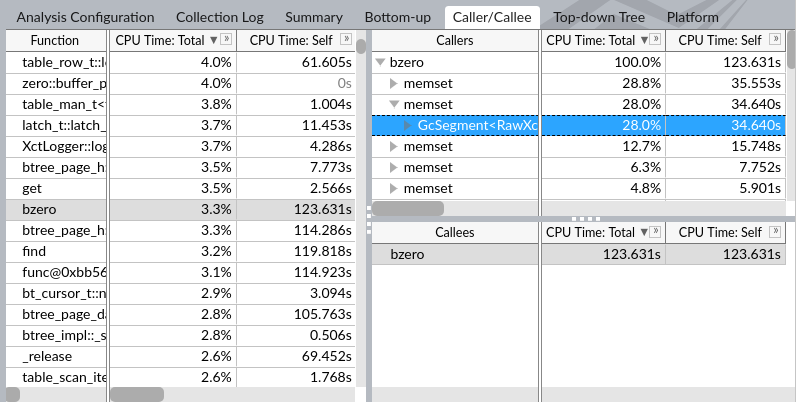
\includegraphics[width = \linewidth]{data/bzero.png}\\
\end{frame}

\begin{frame}
    \frametitle{System Call: bzero}

    \pgfplotsset{%
        every axis/.append style = {
            xlabel = {$\text{Transaction throughput }\left[\si{1\per\minute}\right]$},
            xlabel near ticks,
            x label style = {font = \small},
            xticklabel style = {font = \scriptsize,
                                /pgf/number format/fixed,
                                rotate = 30,
                                align = center},
            xmode = normal,
            xmin = 0,
            scaled x ticks = false,
            xbar = .8pt,
            ymin = -0.75,
            ymax = 1.75,
            bar width = 2.5em,
            ytick style = {draw = none},
            ytick = {0, 1},
            yticklabels = {Optimized, Baseline},
            y tick label style = {align = center,
                                  font = \footnotesize},
            ylabel near ticks,
            y label style = {font = \small},
            xmajorgrids = true,
            width = \textwidth,
            height = .5\paperheight
        }
    }
    \begin{tikzpicture}
        \begin{axis}
            \addplot[draw = Cerulean, fill = Cerulean!50] coordinates
                {(889279.6, 0) (883277.13, 1)};
        \end{axis}
    \end{tikzpicture}
\end{frame}